%
% teil2.tex -- Harmonische Systeme und Rauschen
%
% (c) 2023 Lukas Reitemeier, OST Ostschweizer Fachhochschule
%
% !TEX root = ../../buch.tex
% !TEX encoding = UTF-8
%

\section{Rauschen\label{brown:Rauschen}}
\rhead{Implikationen}

Um dem Thema des Buches gerecht zu werden und dieses Kapitel einzugliedern, kann die harmonische Analysis als essenzielles Werkzeug betrachtet werden. So ist zum Beispiel die \textit{Fast Fourrier Transform} eine wichtige Methode, um periodische Signale von Rauschen zu unterscheiden. So kann bezüglich der Intensität der auftretenden Frequenzen und der Verteilung der Amplituden im Frequenzspektrum, also deren Leistungsdichte, charakterisiert werden. 
So können mittels harmonischer Analysis Filter entwickelt werden, welche ein Signal von Rauschen befreien. Für gewisse Anwendungen ist es auch möglich mit hochfrequenter überlagerten Schwingungen Rauschen zu simulieren. Durch die Analyse von Systemantworten auf verschiedene harmonische Anregungen, kann eine Aussage getroffen werden, wie ein System auf Rauschen --- also eine zufällige konstante Störung --- reagieren würde. 
%Problematisch dabei kann sein, dass je nach Definition und Anwendung \textit{echtes Rauschen} weder vorhersagbar sein sollte, noch Information beinhalten.

%All diese Beispiele basieren auf Methoden der harmonischen Analysis, um den Bogen zur Anfangsbemerkung dieses Kapitels zu schliessen.


\subsection{Was ist Rauschen?\label{brown:Rauschen:Arten}}

\begin{figure}
	\centering
	\begin{minipage}{0.45\textwidth}
		\centering
		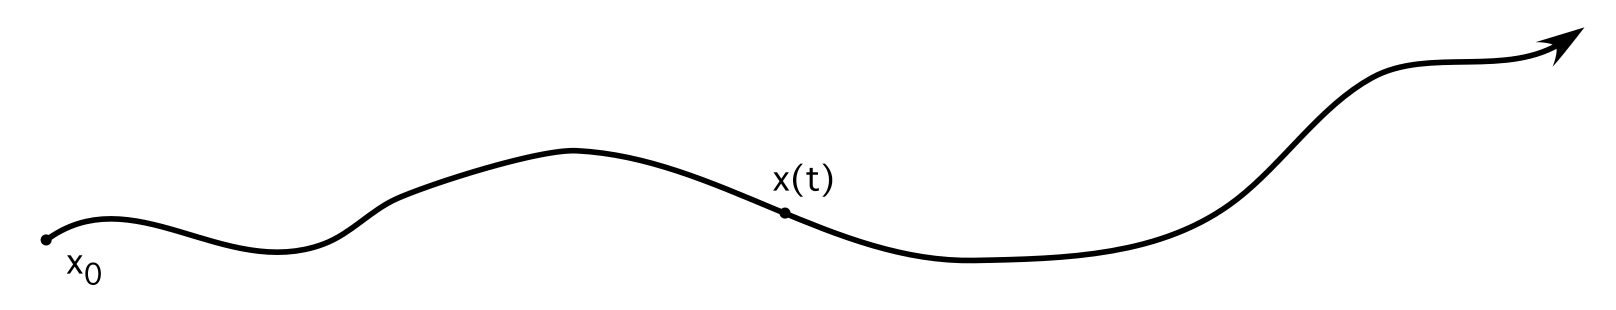
\includegraphics[width=\textwidth]{papers/brown/images/idealSignal.png}
		\caption{Ideales Signal}
		\label{idealSignal}
	\end{minipage}
	%\hspace{0.05\linewidth}
	\begin{minipage}{0.45\textwidth}
		\centering
		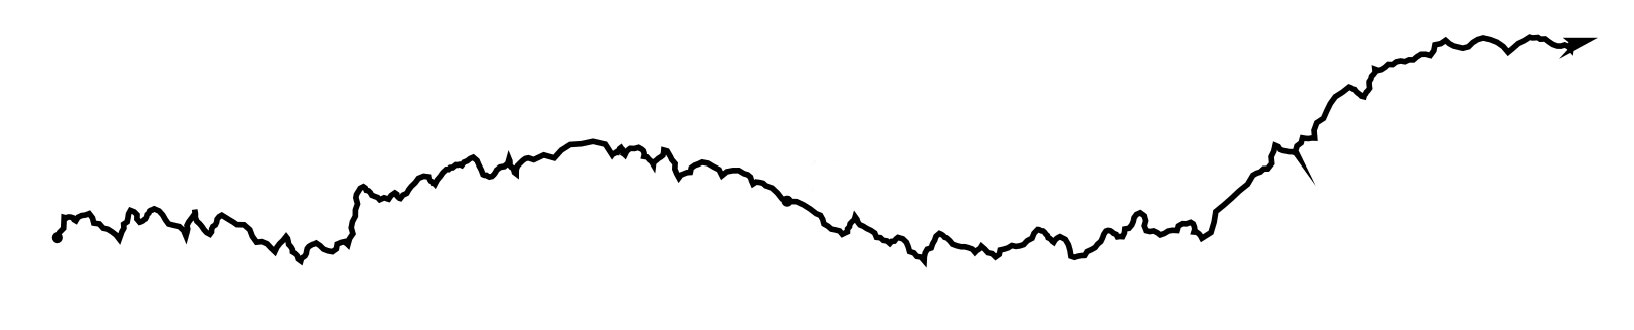
\includegraphics[width=\textwidth]{papers/brown/images/realSignal.png}
		\caption{Reales Signal}
		\label{realSignal}
	\end{minipage}
\end{figure}

Rauschen ist in vielen technischen und wissenschaftlichen Disziplinen ein wichtiger Faktor, so kann es auch in verschiedenen Kontexten unterschiedlich definiert werden. In der Signal- und Kommunikationstechnik ist Rauschen als ungewollte Störung eines Signals definiert. Ein perfektes ungestörtes Signal, wie in Abbildung \ref{idealSignal} gibt es nur in der Theorie. In der Realität sind alle Signale von Rauschen behaftet, wie der Abbildung \ref{realSignal} dargestellt.

Eine solche Störung kann auf einem deterministischen Zusammenhang beruhen oder rein zufälliger Natur sein. Zum Beispiel kann bei elektronischen Messungen durch das Magnetfeld von Stromkabeln eine Störung hervorgerufen werden, dies wäre eine deterministische Störungen (konstant 50 Hz Wechselstrom). Es gibt aber auch rein zufällige Störungen, wie zum Beispiel durch kosmische Teilchen, welche einen Empfänger oder Messgerät beeinflussen können. Wird ein Signal ununterbrochen von Störungen beeinflusst, kann von Rauschen gesprochen werden. Mathematisch können unterschiedliche Arten von Rauschen unterschieden werden, einige der wichtigsten sind folgende: 
% https://www.elektroniktutor.de/elektrophysik/rauschen.html

\begin{definition}{\bf Weisses Rauschen:}
	\begin{itemize}
		\item Die spektrale Leistungsdichte ist konstant über alle Frequenzen. 
	\end{itemize}
\end{definition}


Ein Beispiel dafür ist das Rauschen von Radios, wenn die Frequenz nicht korrekt eingestellt ist, ausgelöst durch Störeinflüsse wie zum Beispiel: Elektrische Interferenzen, kosmische Einflüsse oder auch Blitzentladungen. Analog zu weissem Licht, kann weisses Rauschen so interpretiert werden, dass sich verschiedene Frequenzen überlagern, wobei anzumerken ist, dass weisses Licht keine konstante Leistungsdichte im Spektrum aufweisst.

\begin{definition}{\bf Rosa Rauschen}
	\begin{itemize}
		\item Die Amplituden des Rauschens werden mit zunehmender Frequenz kleiner, sind also invers proportional zur Frequenz $ ~1/f $.
	\end{itemize}
\end{definition}


Um bei einem hörbaren Beispiel zu bleiben: Rosa Rauschen klingt als Schall ausgewogener und ``weicher'' als weißes Rauschen. Dies, da unangenehme hohe Frequenzen wegfallen. Der Begriff ``Rosa'' ist eine Analogie zum sichtbaren Licht, bei dem tiefere Frequenzen auch eher rötlich erscheinen und überlagert mit Weiss (weisses Rauschen), Rosa ergeben. In der Elektronik wird der Abfall der Leistungsdichte mit 3 $ dB $ pro Oktave charakterisiert.

\begin{definition}{\bf Braunes Rauschen (Brownsches Rauschen):}
	\begin{itemize}
		\item Die Leistungsdichte nimmt im Spektrum mit zunehmender Frequenz invers quadratisch ab ($ ~1/f^2 $).
	\end{itemize}
\end{definition}


"Braun" bezieht sich hier nicht auf eine Farbe, sondern ist Robert Brown gewidmet. Denn die Brownsche Modekühlbewegung entspricht diesem Rausch-Typ, da sich die beobachteten trägen Moleküle mit zunehmender Frequenz verstärkt gegenseitig behindern. In der Elektronik wird der Abfall der Leistungsdichte mit 6 $ dB $ pro Oktave charakterisiert.


\begin{definition}{\bf Gaussisches Rauschen:}
	\begin{itemize}
		\item Die Amplituden im Leistungsspektrum weisen eine Normalverteilung (Gaussverteilung) um eine zentrale Frequenz auf.
	\end{itemize}
\end{definition}


Diese Art von Rauschen ist auf digitalen Bildern zu finden deshalb speziell für die digitale Bildverarbeitung relevant. Die örtliche Verteilung des Rauschens im Bild kann über eine Frequenz charakterisiert werden.


\begin{definition}{\bf Impulsrauschen:}
	\begin{itemize}
		\item Plötzliche, unerwartete Spitzen der Amplitude 
		\item Nicht kontinuierlicher Signalverlauf (skalierter Impuls)
		\item Eine unregelmässig verteilte Leistungsdichte
	\end{itemize}
\end{definition}


In der Bildverarbeitung ist diese Art von Rauschen als \textit{salt \& pepper} bekannt. Dabei nehmen einzelne Pixel plötzlich extreme Werte an, sprich extrem schwarz oder weiss. Diese Pixel wirken visuell auf dem Bild wie verstreutes Salz oder Pfeffer.


Natürlich kann noch zwischen vielen weiteren Typen unterschieden werden, doch auf diese wird nicht eingegangen.


\begin{figure}
	\centering
	\begin{minipage}{0.48\textwidth}
		\centering
		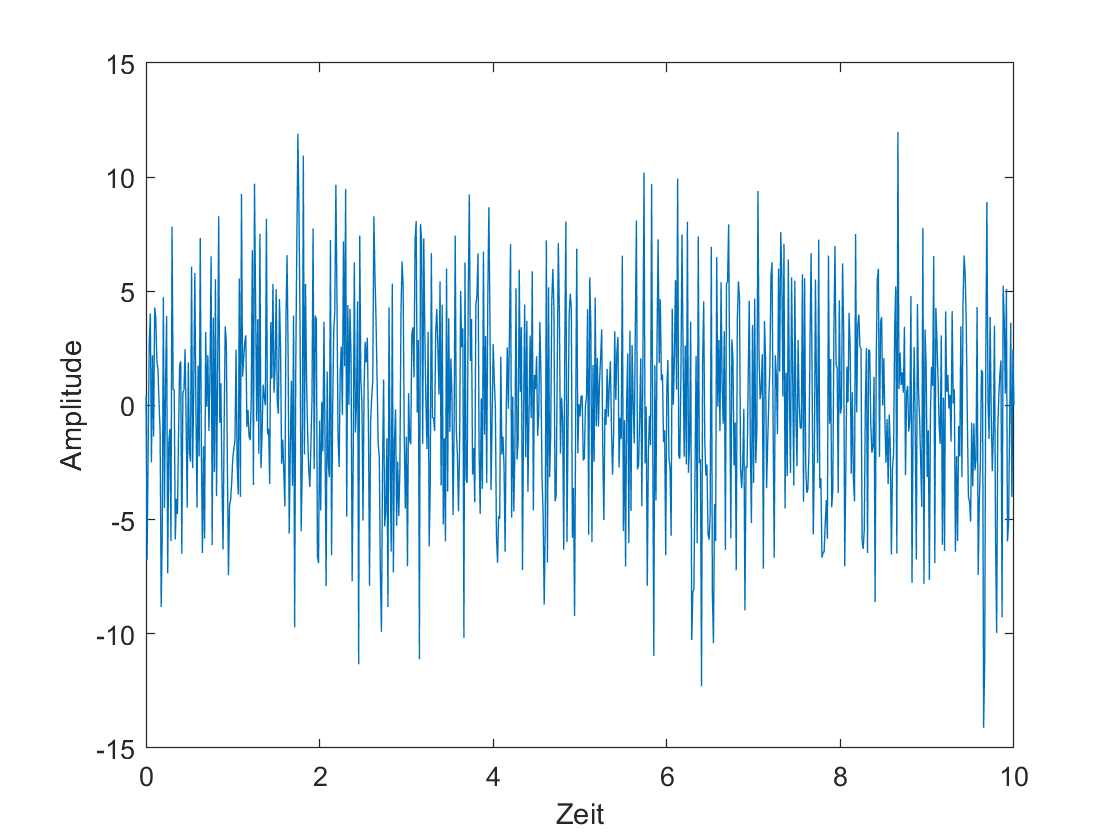
\includegraphics[width=\linewidth]{papers/brown/images/weissesRauschen.png}
		\caption{Echtes weisses Rauschen}
		\label{brown:weissesRauschenSignal}
	\end{minipage}
	%\hspace{0.05\linewidth}
	\begin{minipage}{0.48\textwidth}
		\centering
		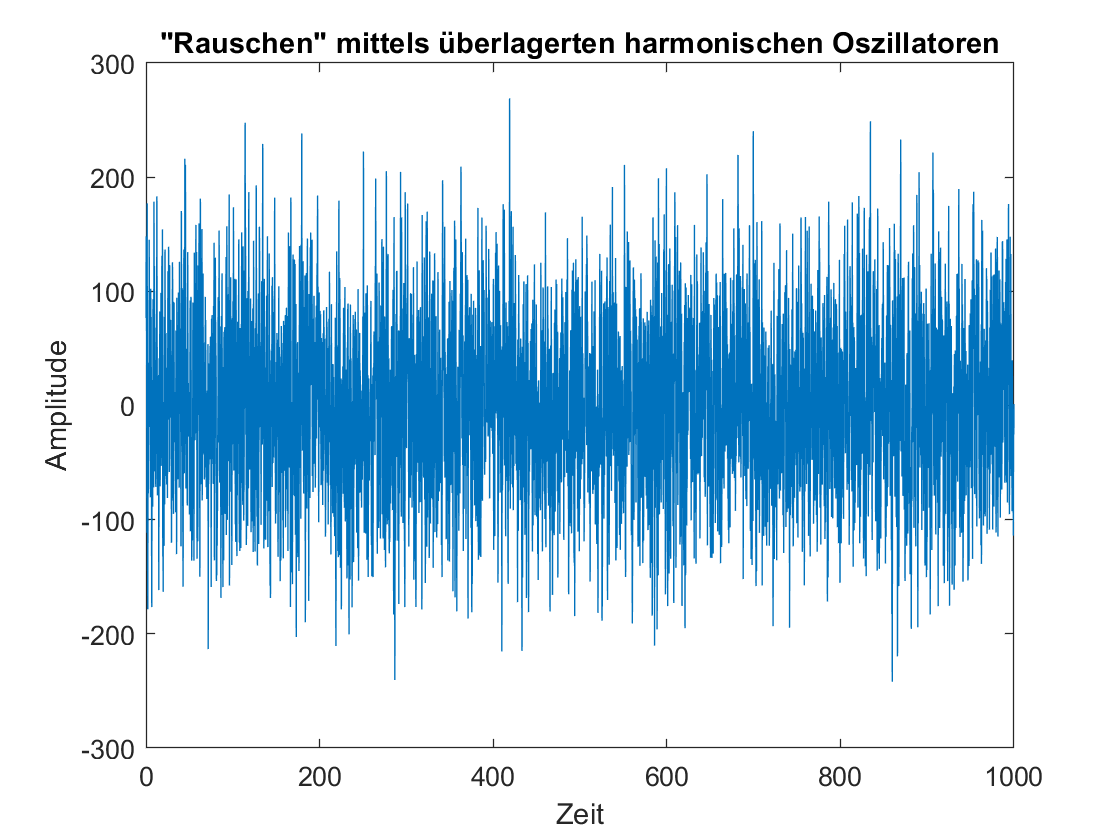
\includegraphics[width=\linewidth]{papers/brown/images/RauschenDurchUeberlagerteHarmonsicheSchwingungen.png}
		\caption{Überlagerte harmonische Schwingungen als Rauschen}
		\label{brown:überlagerteSchwingungen}
	\end{minipage}
	\begin{minipage}{0.48\textwidth}
		\centering
		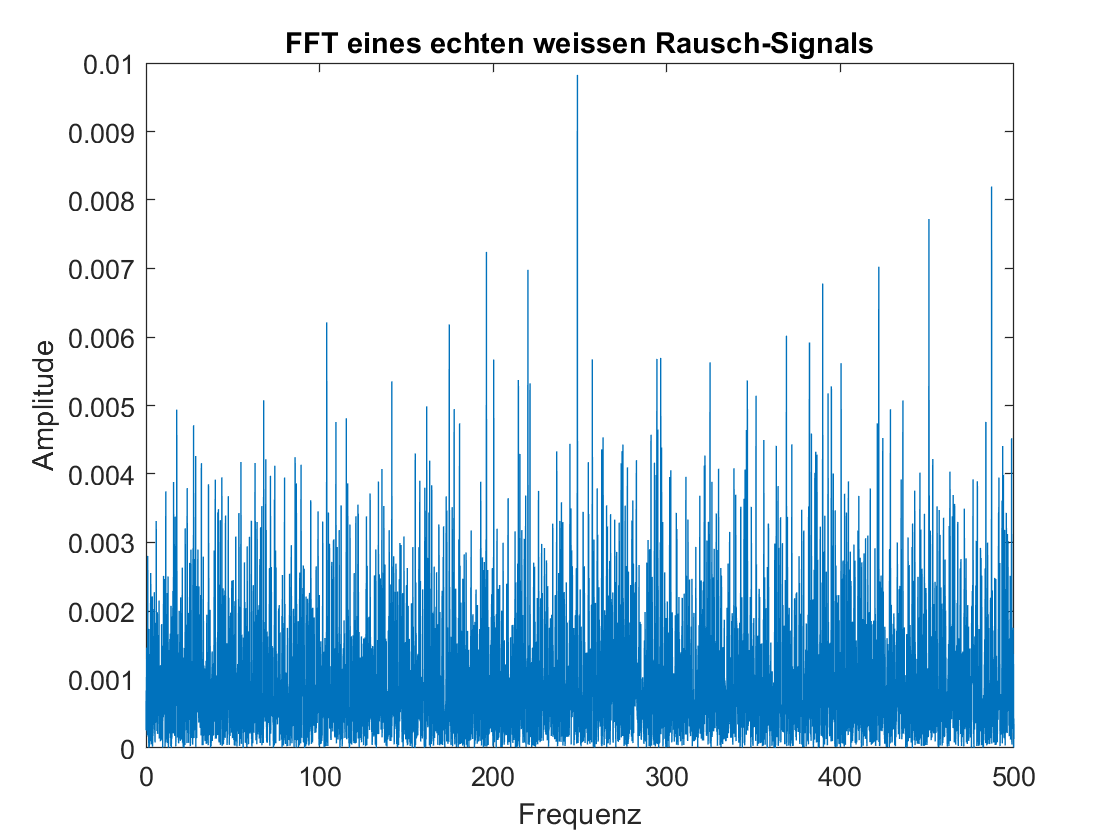
\includegraphics[width=\linewidth]{papers/brown/images/FFTweissesRauschen.png}
		\caption{FFT von weissem Rauschen}
		\label{brown:FFTweissesRauschen}
	\end{minipage}
	%\hspace{0.05\linewidth}
	\begin{minipage}{0.48\textwidth}
		\centering
		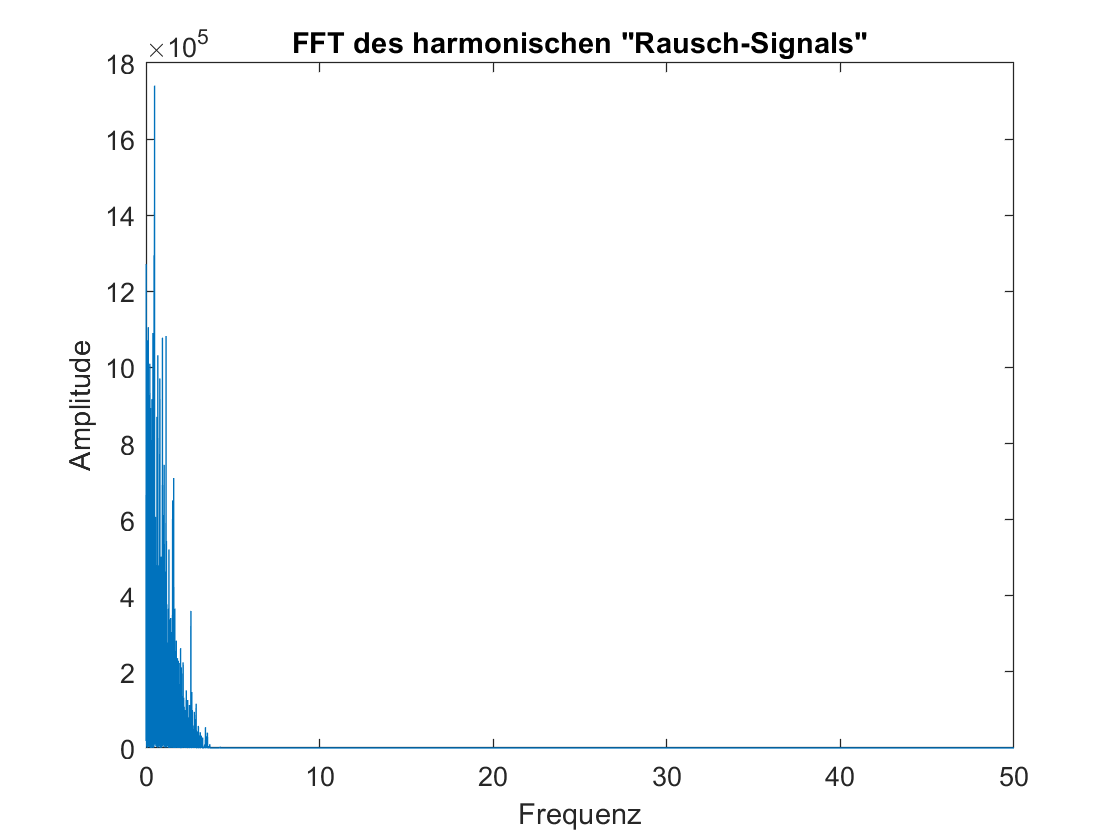
\includegraphics[width=\linewidth]{papers/brown/images/FFT-ueberlagerteSchwingungen.png}
		\caption{FFT von überlagerten harmonischen Schwingungen}
		\label{brown:FFTüberlagerteSchwingungen}
	\end{minipage}
\end{figure}


Viele Signale wirken visuell, wie Rauschen, obwohl sie kaum von einer zufälligen Störungen behaftet sind, sofern nur der zeitliche Verlauf betrachtet wird. So zum Beispiel hochfrequente überlagerte Schwingungen. Diese Überlagerungen sind in der Nachrichtentechnik häufig anzutreffen, als aufmodulierte Signale oder auch überlagerte Signale verschiedener Frequenzen. Aus technischen Gründen kann dies Sinn machen, zum Beispiel um mehr Information über den selben Signalträger zu senden oder das Signale einfacher und robuster zu übertragen.


In den zwei Abbildungen ~\ref{brown:weissesRauschenSignal} und ~\ref{brown:überlagerteSchwingungen} sind zwei Signale aufgetragen, eines stellt echtes stochastisches Rauschen dar, das andere besteht aus vielen hochfrequenten überlagerten Schwingungen. Dieses Beispiel soll verdeutlichen, dass es nicht reicht, nur den zeitlichen Verlauf eines Signals zu betrachten. So könnte man fälschlicherweise die Signale als ähnlich erachten --- eine krasse Täuschung, welche sich im Frequenzspektrum klar zeigt. 



\subsection{Rauschen mittels Wiener-Prozess\label{brown:Rauschen:RandomWalkWiener}}

Um Rauschen zu modellieren, muss als Grundlage ein stochastischer Prozess definiert werden. Zwei weit verbreitete Konzepte dabei sind der \textit{random walk} und der \textit{Wiener-Prozess}.

\begin{definition}\textbf{Random Walk:}
	\label{randomWalk}
	Bei einem Random Walk beginnt man an einem Ausgangspunkt (normalerweise 0) und macht bei jedem Zeitschritt einen zufälligen Schritt vor oder zurück. Oft dient dazu die Binominalverteilung, wobei auch asymmetrische Verteilungen verwendet werden können. Die Schrittlänge und Richtung kann ebenfalls durch eine unabhängige Wahrscheinlichkeitsverteilung bestimmt werden, wobei meist eine konstante Schrittlänge angenommen wird. Dieses Verfahren zeichnet sich durch eine einfache numerische Implementation aus, da es per Definition schon diskret ist.
\end{definition}

\begin{definition}\textbf{Wiener-Prozess:}
	\label{wienerprozess}
	Der Wiener-Prozess ist ein kontinuierlicher stochastischer Prozess, der mit dem Wert 0 startet und unabhängige normalverteilte Änderungen aufweisst. Speziell dabei ist, dass unabhängig von der verstrichenen Zeit der Erwartungswert stets dem Ausgangswert entspricht. Der Wiener-Prozess kann auch als Grenzwert eines Random Walks erachtet werden, sofern die Zeitschritte und Schrittgrössen gegen null gehen und der Prozess bei 0 startet. 
\end{definition}

Beide Prozesse erfüllen die sogenannte \textit{Markov-Eigenschaft}, was bedeutet dass ihre zukünftige Entwicklung nur von ihrer aktuellen Position und nicht von ihrer vergangenen Geschichte abhängt.

Der Wiener-Prozess muss formal also folgende Eigenschaften erfüllen: 

\begin{enumerate}
	\item $ W(0) = 0 $; Der Startwert von $ t = 0 $ ist 0.
	\item $ W(t_{1}) - W(t_{2}) $ ist ein normalverteilte Zufallsvariable mit Erwartungswert 0 und Varianz $ t_{1} - t_{2} $.
	\item Zu jedem weiteren Zeitpunkt $ t_{n} $ ist die Zufalls-Variable unabhängig von allen vorhergehenden Werten. Dies wird auch die Markow-Eigenschaft genannt, wenn der Übergang in einen neuen Zustand nicht vom vorherigen Verlauf abhängt.
\end{enumerate}

Genauer wird auf den Wiener-Prozess nicht eingegangen, da dieser ausführlich im Kapitel \textit{8.1 Modell für Rauschen: der Wiener-Prozess} des Buches \cite{brown:Differenzialgleichungen} vom Mathematischen Seminar über Differenzialgleichungen beschrieben wird.


Nun, da der Wiener-Prozess definiert ist, soll versucht werden weisses Rauschen zu simulieren. Dafür eignet sich der Wiener-Prozess perfekt, denn die Differenzierung des Wiener-Prozesses

\begin{equation}
	\xi(t) = \frac{dW(t)}{dt}
\end{equation}

ergibt direkt weisses Rauschen. Erklärt werden kann dies anhand der Definition. Die Änderungen sind rein zufällig und normalverteilt, so ergibt sich ein gleichmässiges Frequenzspektrum der Änderungsraten.

%Da der in der Abbildung \ref{brown:1Dbrownian} dargestellte Börsen-Verlauf nichts anderes als der Wiener-Prozess mit Drift-Komponente ist, sollte weisses Rauschen durch dessen Differenzierung generiert werden können. In der Abbilung \ref{...} wurde das Frequenzspektrum des simulierten Börsenkurses berechnet. 

Im der Abbildung \ref{brown:WienerProzessFFT} ist die Simulation eines Wiener-Prozesses, also einer brownschen Bewegung, und dessen Frequenzspektrum aufgetragen. Der Unterschied zum simulierten Börsenkurs in der Abbildung \ref{brown:1Dbrownian} ist lediglich, dass keine absichtliche Drift-Komponente miteinbezogen wurde. Man kann feststellen, dass die Leistungsdichte mit zunehmender Frequenz abnimmt. Dies bedeutet, dass tiefe Frequenzen sich im Signal stärker äussern als hohe, also mehr Energie beinhalten. Nun kann die brownsche Bewegung in im Frequenzbereich mittels einer Multiplikation mit der Frequenz $ jwt $ differenziert werden. Es ergibt sich ein konstante Leistungsdichtespektrum. Durch eine inverse Fourriertransformation erhält man wieder ein Signal in der Zeitdomäne. Dieses besteht ausschliesslich aus weissem Rauschen, wie in der Darstellung \ref{brown:diffWienerFFT} zu sehen ist.

%ToDo: Alles in eine Grafik und übereinander gross darstellen
\begin{figure}
	\centering
	\begin{minipage}{0.48\textwidth}
		\centering
		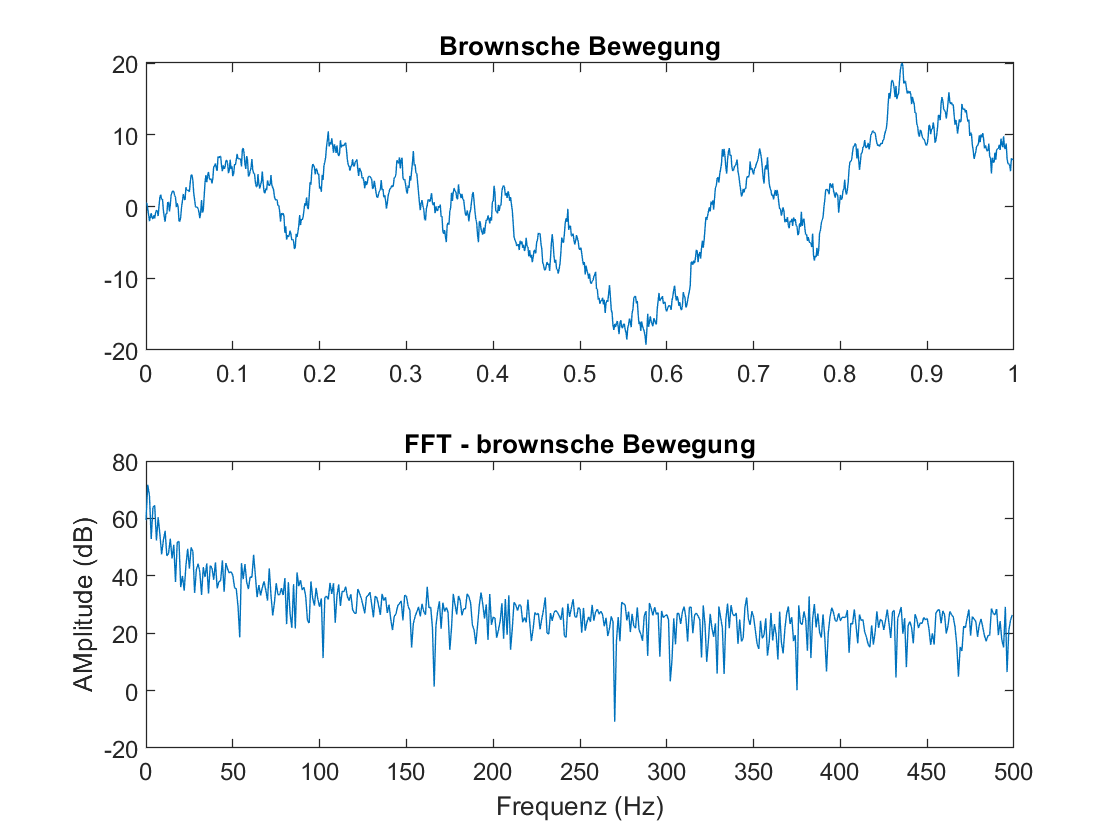
\includegraphics[width=\linewidth]{papers/brown/images/brownscheBewegungUndFFT.png}
		\caption{Wiener-Prozess und Frequenzspektrum}
		\label{brown:WienerProzessFFT}
	\end{minipage}
	%\hspace{0.05\linewidth}
	\begin{minipage}{0.48\textwidth}
		\centering
		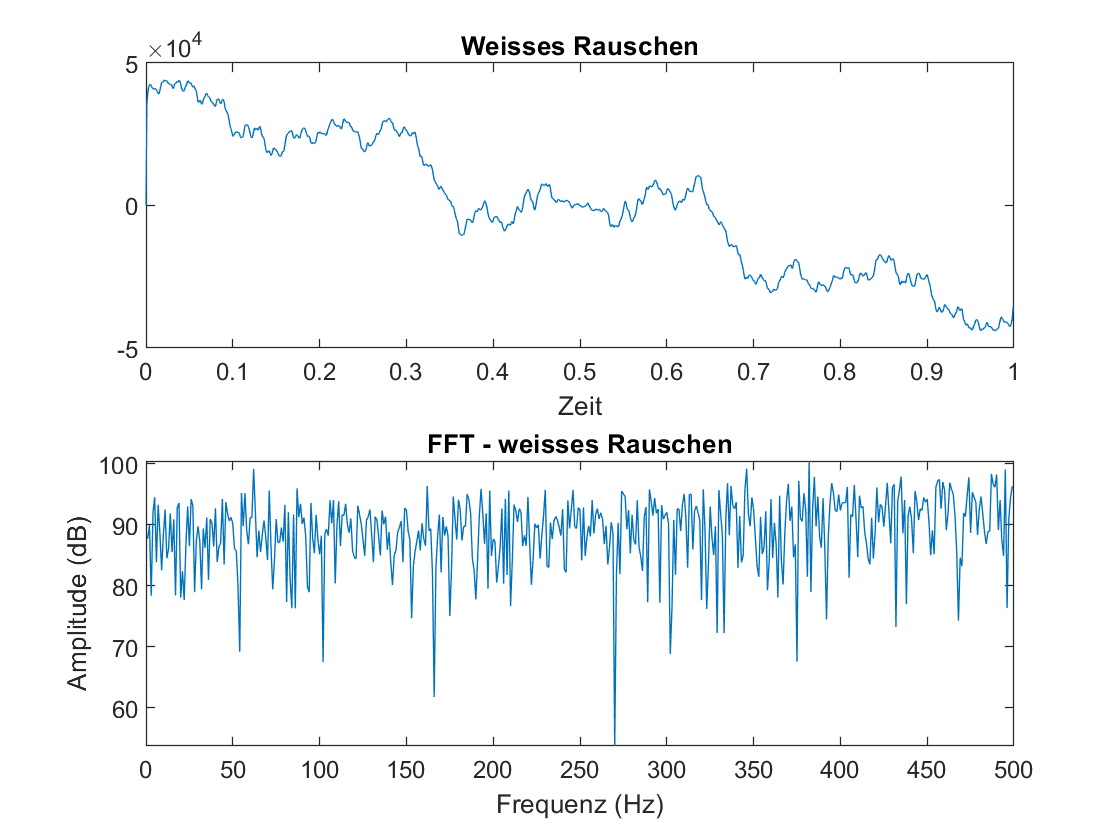
\includegraphics[width=\linewidth]{papers/brown/images/weissesRauschenDurchBrownUndFFT.png}
		\caption{differenzierter Wiener-Prozess und Frequenzspektrum}
		\label{brown:diffWienerFFT}
	\end{minipage}
\end{figure}


\subsection{Implikationen\label{brown:Rauschen:Implikationen}}

Ein grosses Problem im Zusammenhang mit Rauschen, ist die Differenzierbarkeit. Dies ist häufig beim Umgang mit Mess-Signalen der Fall, was das bestimmen einer lokalen Steigung erschwert und die Äderungsrate verfälscht. Davon sind auch empfangene Datensignale betroffen, was zu falsch dekodierten Informationen führen kann. Die einfachste Methode und häufig ein erster Schritt in der Signalverarbeitung, ist die Anwendung eines Tiefpass- oder Bandpass-Filters. Dieser entfernt jedoch nicht nur das Rauschen, sondern auch ein Teil der im Signal enthaltenen Information.

Eine weitere Schwierigkeit entsteht, wenn anhand von Messdaten ein Modell erstellt werden soll, welches das Verhalten der Messdaten widerspiegelt. Dabei kann es sein, dass man das Rauschen als Teil des Systems identifiziert oder rein als externe Störung. Im einen Fall muss dann zwischen System und Rauschen unterschieden werden, im anderen Fall muss das System selbst Rauschen abbilden können.
% Absatz?

Ist ein System anhand einer gewöhnlichen Differenzialgleichung (DGL) gegeben, kann das Verhalten des Systems unter Berücksichtigung der Anfangsbedingungen vorhergesagt werden. Vom Anfangswert aus entwickelt sich die Funktion gemäss der Startbedingung und dem durch die DGL gegebenen Vektorfeld. In vielen Bereichen entspricht ein solch deterministisches System jedoch nicht der Realität und suggeriert eine Aussagekraft, welche sich nicht mit Beobachtungen deckt. Es gibt Systeme, welche stark auf kleine Störeinflüsse reagieren. Dies führt dazu, dass sich die Lösung einer DGL gegenüber der Realität, zum Beispiel durch Rauschen, nicht perfekt deckt oder das Resultat sogar komplett divergiert. Ein anschauliches Beispiel dafür das System,

\begin{align}
	\frac{dx}{dt} &= -y \\
	\frac{dy}{dt} &= x^2 + y
	\label{brown:divergentEquation}
\end{align}

für welches in der Abbildung~\ref{brown:divergentAndConvergentSystem} zwei unterschiedliche Trajektorien im Vektorfeld eingezeichnet sind. In rot ist der Verlauf im Intervall  $ t = [0, 3] $ mit dem Startwert $ (-1.7, -1.4) $ aufgetragen und in grün mit dem Startwert $ (-1.8, -1.4) $.

\begin{figure}
	\centering
	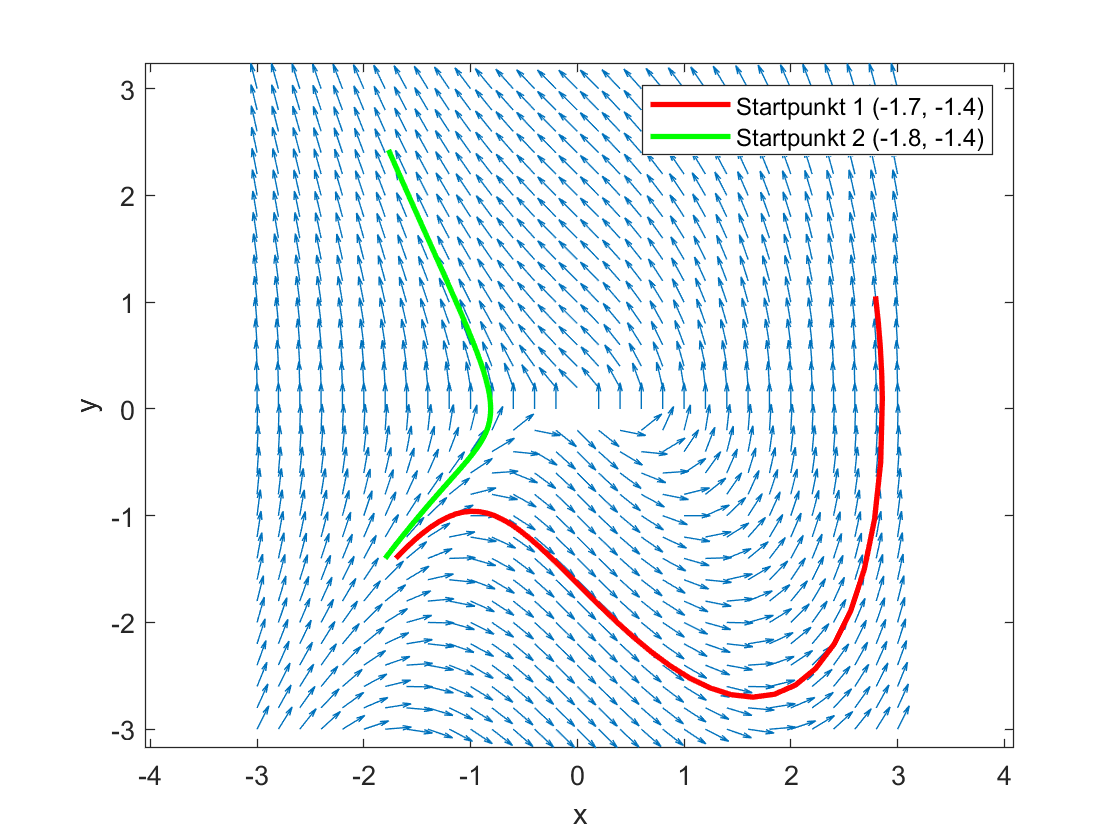
\includegraphics[width=0.8\textwidth]{papers/brown/images/Vektorfeld-mit-zwei-Pfaden.png}
	\caption{Zwei Pfade mit fast gleichem Startpunkt}
	\label{brown:divergentAndConvergentSystem}
\end{figure}

Dieses System veranschaulicht schön, wie sich eine kleine Variation der Startbedingung auf den Verlauf der Lösung auswirken kann. In diesem speziellen Fall konvergieren die Lösung zu einem späteren Zeitpunkt $ t $ wieder. Bedenkt man nun aber, dass eine solche Störung durch Rauschen herbeigeführt werden könnte, scheint es unsinnig, eine einzige fixe Lösung für ein solches System anzugeben --- zumindest nicht ohne auf die Aussagekraft der Lösung unter Rauscheinfluss hinzuweisen oder den Lösungsraum genauer zu spezifizieren.

Es gibt auch Systeme, welche bei kleinen Störungen aus einem stabilen Zustand in einen instabilen Zustand übergehen und komplett divergieren. In solchen Fällen kann es ein fataler Fehler sein, zufällige Störungen des Systems nicht zu berücksichtigen. Andere Systeme beinhalten selbst eine zufällige Komponente, welche nicht vernachlässigt werden soll.

Um diesem Umstand gerecht zu werden, kann man die Möglichkeit von zufälligen Störungen beim Aufstellen eines Modells miteinbeziehen. Anstatt eine fixe Lösung zum Zeitpunkt $ t $ anzugeben, kann man eine Wahrscheinlichkeitsverteilung über die verschiedenen möglichen Endzustände angeben --- et. voilà, man hat den Lösungsraum einer stochastische Differenzialgleichung (SDGL).
